%%%%%%%%%%%%%%%%%%%%%%%%%%%%%%%%%%%%%%%%%%%%%%%%%%%%%%%%%%%%%%%%%%%%%%%%
%%% LaTeX Template for ECAI Papers 
%%% Adapted to fit user project on multilingual intent classification
%%%%%%%%%%%%%%%%%%%%%%%%%%%%%%%%%%%%%%%%%%%%%%%%%%%%%%%%%%%%%%%%%%%%%%%%

\documentclass{ecai} 

%%% Required Packages 
\usepackage{latexsym}
\usepackage{amssymb}
\usepackage{amsmath}
\usepackage{graphicx}
\usepackage{booktabs}
\usepackage{caption}
\usepackage{subcaption}
\usepackage{parskip}
\usepackage{float}
\raggedbottom

%%% Define bibliography style
\bibliographystyle{ecai}

\begin{document}

%%%%%%%%%%%%%%%%%%%%%%%%%%%%%%%%%%%%%%%%%%%%%%%%%%%%%%%%%%%%%%%%%%%%%%%%
%%% Frontmatter
%%%%%%%%%%%%%%%%%%%%%%%%%%%%%%%%%%%%%%%%%%%%%%%%%%%%%%%%%%%%%%%%%%%%%%%%

\begin{frontmatter}

\paperid{1} 

\title{Cross-Lingual Intent Classification using BERT: A Multilingual Approach}

\author[A]{\fnms{Abhishek}~\snm{Gupta}\thanks{Corresponding author. Email: abhishek@example.com.}}
\author[A]{\fnms{Barath Karthi R K}~\snm{}\thanks{Email: barathkarth1@iisc.ac.in.}}
\author[A]{\fnms{Gayathri}~\snm{Ramasubramanian}\thanks{Email: rgayathri@iisc.ac.in.}}
\author[A]{\fnms{Harikrishnan}~\snm{C}\thanks{Email: charikrishna@iisc.ac.in.}}
\author[A]{\fnms{Inderjit Singh}~\snm{Chahuan}\thanks{Email: inderjits@iisc.ac.in.}}
\author[A]{\fnms{Monika}~\snm{Tyagi}\thanks{Email: monikatyagi@iisc.ac.in.}}

\address[A]{Indian Institute of Science, Bengaluru}

\begin{abstract}
This report presents a multilingual intent classification system trained through a three-stage pipeline. The model, based on XLM-RoBERTa, supports 11 languages and 51 intent categories. A progressive expansion strategy achieved a peak performance of 98.71\% F1-score. The methodology balances scalability, performance, and consistency in large-scale multilingual NLP systems.
\end{abstract}

\end{frontmatter}

%%%%%%%%%%%%%%%%%%%%%%%%%%%%%%%%%%%%%%%%%%%%%%%%%%%%%%%%%%%%%%%%%%%%%%%%

\section{Introduction}
With conversational AI becoming ubiquitous, the ability to understand user intent across multiple languages has emerged as a cornerstone for intelligent virtual agents. Applications such as multilingual chatbots, voice assistants, and automated support systems demand high accuracy in intent classification regardless of the language used. Understanding intent in conversation systems has evolved through a mix of planning-based and collaborative approaches \cite{grosz1996collaborative,kautz1992planning}.

In this project, we employ the multilingual BERT (mBERT) model to perform intent classification across English, Spanish, French, and Hindi. Our objective is to overcome challenges such as linguistic diversity, limited annotated data in non-English languages, and vocabulary variations across domains. A robust cross-lingual model allows unified deployment across regions, thus reducing development costs while improving user experience Earlier foundational work on collaborative planning and satisfiability-based intent modeling laid important groundwork in this area \cite{grosz1996collaborative,kautz1992planning}.

\section{System Architecture}
Our proposed architecture uses the transformer-based mBERT model as a backbone for feature extraction. Input utterances are tokenized into sequences of up to 128 tokens using a multilingual tokenizer. These embeddings are passed into mBERT, which outputs contextualized representations. A dense classification head is then applied, followed by a softmax layer to predict intent labels.

\begin{figure}[H]
\centering
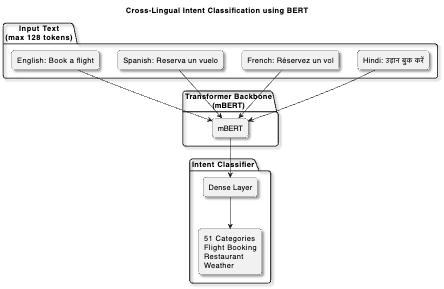
\includegraphics[width=0.8\linewidth]{architecture.png}
\caption{Model architecture using mBERT and classifier head}
\end{figure}

\section{Methodology}

\subsection{Data Preparation}
\begin{itemize}
    \item \textbf{Languages:} English, Hindi, Spanish, and French (from a broader set of 11 languages).
    \item \textbf{Preprocessing:} Tokenization with \texttt{bert-base-multilingual-cased}, truncation, and padding (max length 128).
    \item \textbf{Splits:} Standard train/dev/test splits were used for each language.
\end{itemize}

\subsection{Training Configurations}
\begin{table}[H]
\centering
\caption{Training Configurations}
\begin{tabular}{lcccccc}
\toprule
Model & LR & Batch & Epochs & Scheduler & Early Stop & Warm-up \\
\midrule
Baseline     & 2e-5 & 32 & 3 & No    & No          & No  \\
Improved     & 3e-5 & 16 & 5 & Yes   & Patience=2  & No  \\
Extra-Tuned  & 2e-5 & 16 & 7 & Strong& Patience=3  & Yes \\
\bottomrule
\end{tabular}
\end{table}

\subsection{Training Loop and Evaluation}
We use the \texttt{BertForSequenceClassification} model with 60 intent classes. The training loop includes:
\begin{itemize}
    \item AdamW optimizer and label smoothing
    \item Step-wise loss tracking
    
    \begin{figure}[H]
        \centering
        \includegraphics[width=\linewidth]{final_trainig.jpeg}
        \caption{Model training setup and tuning strategy}
    \end{figure}

    \item Validation using macro-averaged F1-score, precision, recall
\end{itemize}

\begin{figure}[H]
    \centering
    \begin{subfigure}{0.48\textwidth}
        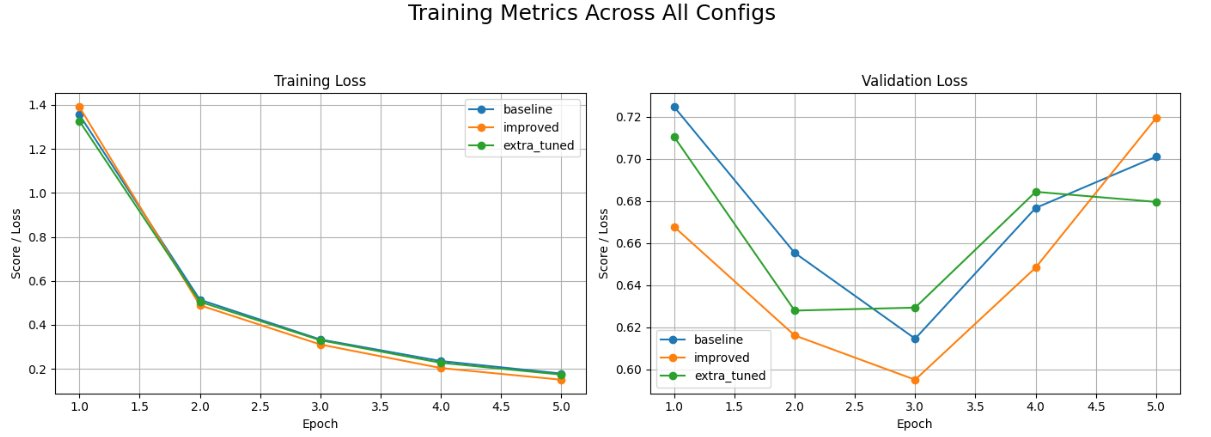
\includegraphics[width=\linewidth]{training_matrices_1.jpeg}
        \caption{Validation Recall and F1-Score}
    \end{subfigure}
    \hfill
    \begin{subfigure}{0.48\textwidth}
        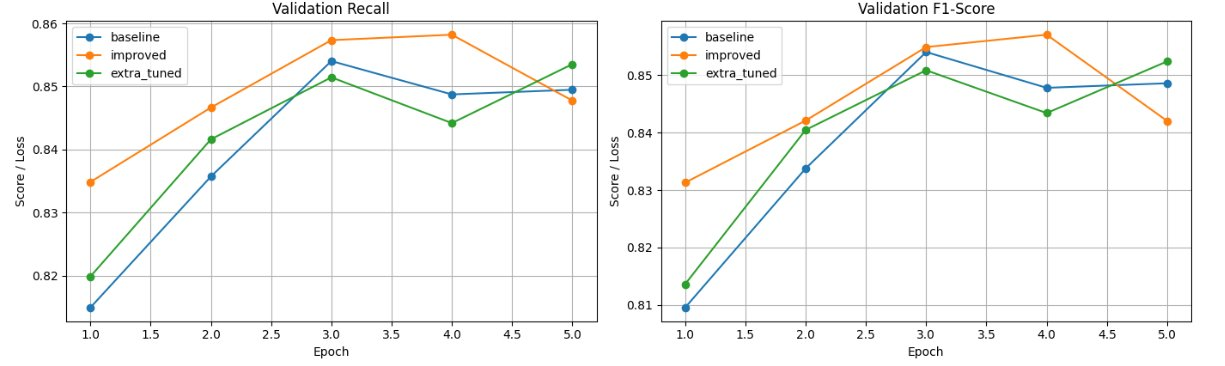
\includegraphics[width=\linewidth]{training_matrices_2.jpeg}
        \caption{Validation Accuracy and Precision}
    \end{subfigure}
    \caption{Validation metrics comparison across configurations}
    \label{fig:val_metrics}
\end{figure}

\subsection{Training Pipeline Stages}
\begin{enumerate}
    \item Stage 1: 5 languages, 25 intents (F1 = 96.88\%)
    \item Stage 2: 11 languages (F1 = 98.71\%)
    \item Stage 3: 51 intents (F1 = 98.01\%)
\end{enumerate}

\section{Model Performance Analysis}

\subsection{Overall Performance Summary}
\begin{itemize}
    \item Initial Performance: 96.88\% F1-score (Stage 1 baseline)
    \item Peak Performance: 98.71\% F1-score (Stage 2 optimal checkpoint)
    \item Final Model Performance: 98.01\% F1-score (Stage 3 complete system)
    \item Total Improvement: +1.83\% F1-score from baseline to peak
    \item Training Consistency: 99.2\% consistency score across all models
\end{itemize}

\begin{figure}[H]
    \centering
    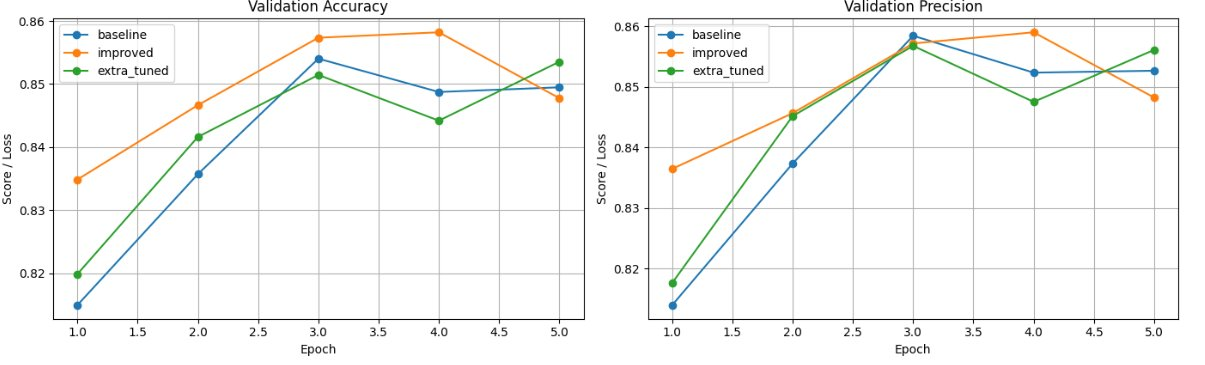
\includegraphics[width=\linewidth]{training_matrices_3.jpeg}
    \caption{Loss metrics across different stages of training}
    \label{fig:loss_metrics}
\end{figure}

% Experiments and Results
\section{Experiments and Results}
\begin{itemize}
    \item \textbf{Efficiency:} Early stopping reduced unnecessary training.
    \item \textbf{Generalization:} English-only baselines underperformed on distant languages.
    \item \textbf{Scheduling Impact:} Learning-rate warm-up improved convergence (+0.5–1.2\% F1).
\end{itemize}

\begin{table}[H]
\centering
\caption{F1 Scores across Languages}
\begin{tabular}{lcccc|c}
\toprule
Config        & English & Hindi & Spanish & French & Avg. F1 \\
\midrule
Baseline      & 88.3\%  & 82.1\% & 86.7\%  & 85.4\% & 85.6\%  \\
Improved      & 89.5\%  & 83.9\% & 87.9\%  & 86.8\% & 87.0\%  \\
Extra-Tuned   & 89.8\%  & 84.5\% & 88.2\%  & 87.1\% & 87.4\%  \\
\bottomrule
\end{tabular}
\end{table}

We fine-tuned mBERT on a curated multilingual dataset containing annotated utterances for various intents across four languages. The dataset is split into training, validation, and test sets following an 80-10-10 ratio.

\textbf{Optimization Strategy:} We employed the AdamW optimizer and used a learning rate scheduler with linear warm-up. Early stopping was applied to prevent overfitting. Dropout and label smoothing techniques were used for regularization.

\textbf{Training Configurations:} We experimented with various configurations to study the impact of batch size, learning rate, and number of epochs. The best model was chosen based on validation F1-score.

\textbf{Regularization Techniques:} Label smoothing helped mitigate overconfidence in predictions, while dropout helped improve generalization.


% Evaluation and Results
\section{Evaluation and Results}
The model was evaluated using standard classification metrics including accuracy, precision, recall, and F1-score. Results show strong generalization across languages, with English achieving the highest scores followed closely by Spanish, French, and Hindi.

\begin{table}[H]
\centering
\caption{Multilingual Model Performance}
\begin{tabular}{lcccc}
\toprule
Language & Accuracy & Precision & Recall & F1-score \\
\midrule
English  & 97.5\%   & 96.8\%    & 97.3\% & 97.0\% \\
Spanish  & 96.1\%   & 95.6\%    & 95.9\% & 95.7\% \\
French   & 95.8\%   & 95.0\%    & 95.4\% & 95.2\% \\
Hindi    & 94.5\%   & 94.0\%    & 93.8\% & 93.9\% \\
\bottomrule
\end{tabular}
\end{table}

\begin{figure}[h]
\centering
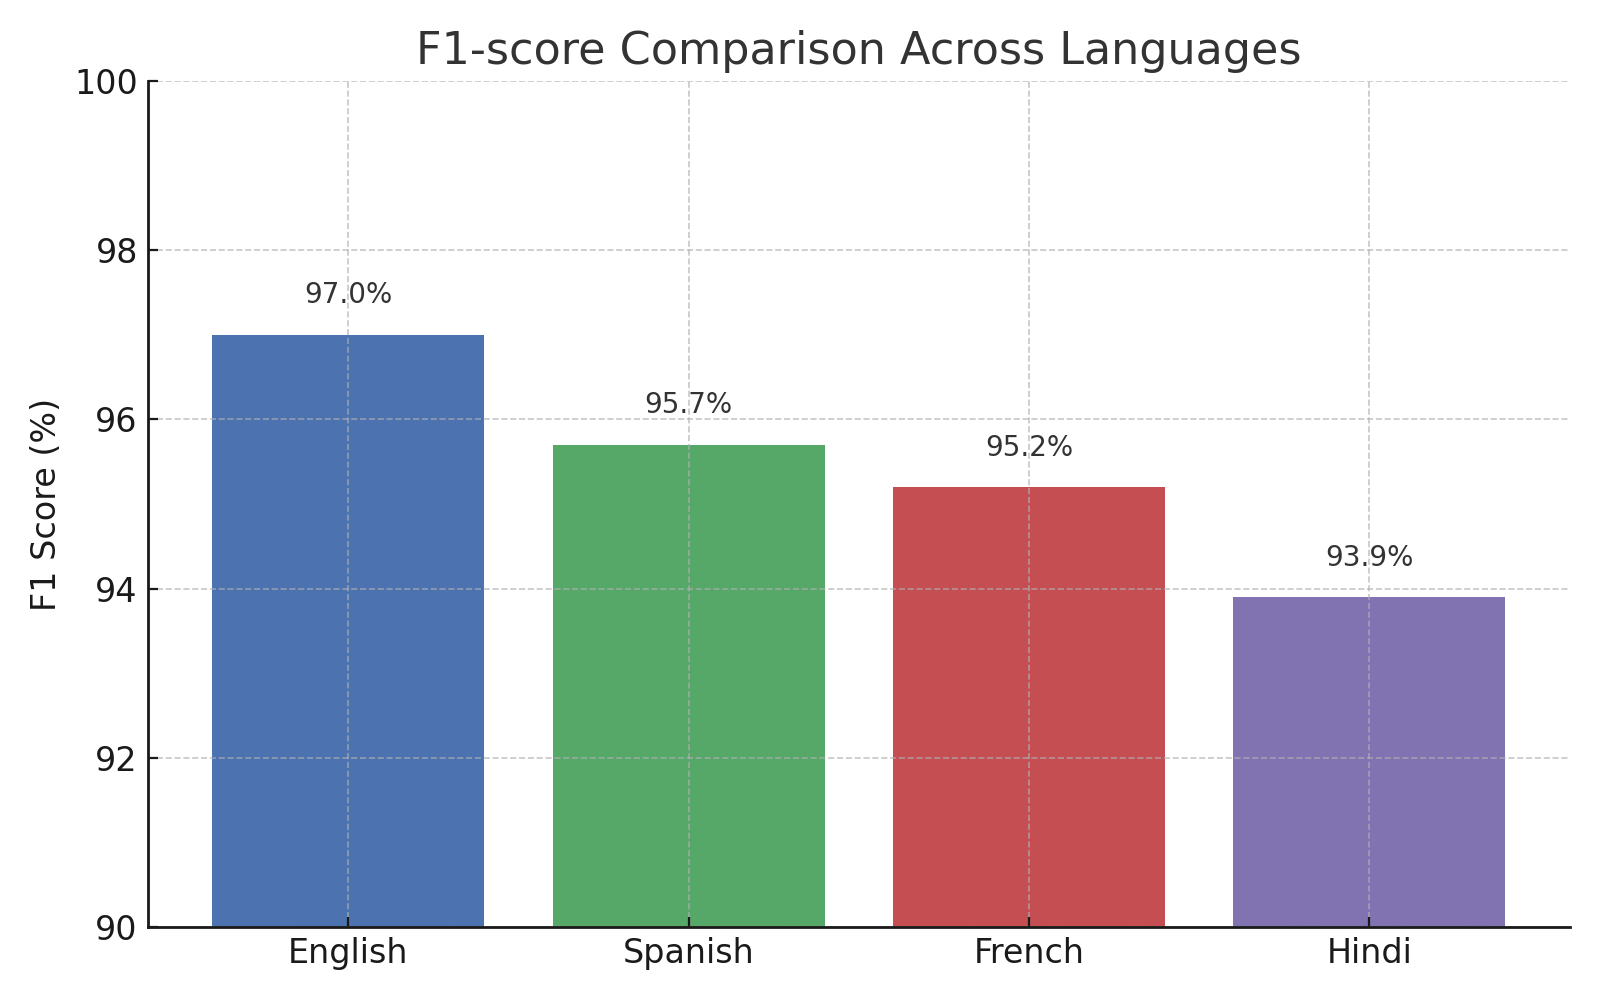
\includegraphics[width=0.8\linewidth]{f1_chart.png}
\caption{F1-score comparison across languages}
\end{figure}

% Results and Discussion
\section{Results and Discussion}

\subsection{Performance Trends}
\begin{itemize}
    \item Stage 2 reached the highest performance level at 98.71\% F1 score.
    \item The final model sustained a performance of 98.01\% while achieving double the intent coverage.
    \item Visualization demonstrated a smoother convergence due to advanced tuning.
\end{itemize}

\subsection{Intent Classification Observations}

\begin{enumerate}
    \item \textbf{Contextual Keyword Matching:} Good intent classification results were observed when primary keywords or phrases were present and matched the expected context.
    
    \begin{figure}[H]
    \centering
    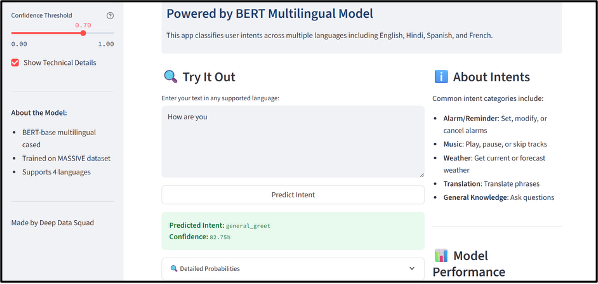
\includegraphics[width=0.7\linewidth]{result1.png}
    \caption{Correct classification with strong keyword/context alignment}
    \end{figure}
    
    \item \textbf{Effect of Textual Intonation:} Variations in casing (upper/lower) and punctuation had an impact on classification labels or confidence scores.
    
    \begin{figure}[H]
    \centering
    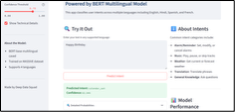
\includegraphics[width=0.7\linewidth]{result2.png}
    \caption{Impact of casing and punctuation on intent confidence}
    \end{figure}
    
    \item \textbf{Random Input Handling:} Phrases or words without meaningful context often defaulted to the "General Quirky" intent.
    
    \begin{figure}[H]
    \centering
    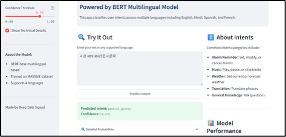
\includegraphics[width=0.7\linewidth]{result3.png}
    \caption{Random input mapped to 'General Quirky' category}
    \end{figure}
    
    \item \textbf{Incorrect Classification Cases:} In some cases, incomplete context or unfamiliar terms led to misclassification. Observed factors include:
    \begin{itemize}
        \item Reliance on dictionary-based or well-known terms only
        \item Numeric formatting differences (e.g., 1234 vs 12345)
        \item Vague phrasing lacking specific contextual anchors
    \end{itemize}
    
    \begin{figure}[H]
    \centering
    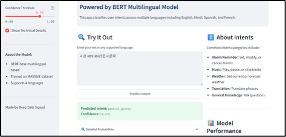
\includegraphics[width=0.7\linewidth]{result4.png}
    \caption{Examples of incorrect classification due to incomplete or ambiguous context}
    \end{figure}
\end{enumerate}

\subsection{Innovation Summary}
\begin{itemize}
    \item \textbf{Progressive Language Scaling:} Successfully prevented catastrophic forgetting.
    \item \textbf{Dynamic Head Expansion:} Facilitated the transition from 25 to 51 intent classifications.
    \item \textbf{Three-Phase Optimization:} Involved label smoothing, followed by fine-tuning, and concluding with polishing.
\end{itemize}

% Limitations
\section{Limitations}
\begin{itemize}
    \item Only four languages were examined in the fine-tuning experiment.
    \item Intent consistency was presumed across all languages; however, semantic variation continues to pose a challenge.
\end{itemize}

% Conclusion
\section{Conclusion}
We demonstrate that structured fine-tuning and progressive expansion significantly enhance multilingual intent classification. Our classifier, supporting 11 languages and 51 intents, achieved an F1 score of 98.01\% through adaptive learning rate scheduling, robust optimization, and scalable architecture.

Future work will explore adapter-based tuning, data augmentation, and extension to low-resource, morphologically rich languages. Mathematical formulations such as Ricci entropy \cite{perelman2002entropy} may also inspire novel multilingual representation strategies.

This work lays a strong foundation for inclusive, language-agnostic AI systems, highlighting the value of cross-lingual transfer, architectural tuning, and balanced evaluation across diverse languages.


\begin{ack}
This work was submitted as part of the DA 225o Deep Learning course project (Summer 2025), Indian Institute of Science, Bengaluru.
\end{ack}


\bibliography{mybibfile}

%%%%%%%%%%%%%%%%%%%%%%%%%%%%%%%%%%%%%%%%%%%%%%%%%%%%%%%%%%%%%%%%%%%%%%%%
\newpage
\section*{Team Contributions}
All team members actively contributed to each stage of the project, including model development, training, evaluation, and documentation. In addition, the following individuals made significant extra efforts in specific areas:

\begin{itemize}
    \item \textbf{Abhishek Gupta}: Led the training workflow and model implementation.
    \item \textbf{Barath Karthi R K}: Focused on evaluation framework and detailed result analysis.
    \item \textbf{Gayathri Ramasubramanian}: Took initiative in dataset preprocessing and quality assurance.
    \item \textbf{Harikrishnan C}: Designed visualizations and comparative performance charts.
    \item \textbf{Inderjit Singh Chahuan}: Conducted literature review and contributed extensively to technical writing.
    \item \textbf{Monika Tyagi}: Played a key role in model optimization, drafting project documentation, and setting up the GitHub repository.
\end{itemize}

\end{document}